\documentclass[12pt]{report}
\usepackage[utf8]{inputenc}
\usepackage{graphicx}
\usepackage{geometry}
  \geometry{
    left =25mm,
    right = 25mm
  }

\linespread{1.3}
\usepackage{tikz}
\usetikzlibrary{arrows, shapes, positioning}

\graphicspath{{images/}}

\usepackage{amsthm}
\usepackage{amsmath}
\usepackage{amsfonts}
\usepackage{algorithmic}
\usepackage{algorithm}

\newtheorem{thm}[algorithm]{Theorem}
\newtheorem{definition}[algorithm]{Definition}
\newtheorem{cor}[algorithm]{Corollary}
\newtheorem{conj}[algorithm]{Conjecture}
\newtheorem{remark}[algorithm]{Remark}
\newtheorem{claim}[algorithm]{Claim}
\newtheorem{lemma}[algorithm]{Lemma}
\newtheorem{guess}[algorithm]{Statement}
\newtheorem*{conj*}{Conjecture}

\begin{document}
\begin{titlepage}
  \begin{center}
    \textsc{
      \large
      Eötvös Loránd University \\
      Faculty of Science \\
    }
    \vspace{0.4cm}

    \rule{14cm}{0.4pt}
    \vspace*{1.2cm}

    \LARGE{Hanna Gábor}

    \huge
    \vspace{0.6cm}
    \textbf{Super-duper Thesis Title} \\
    \vspace{0.3cm}
    \normalsize
    Diploma Thesis \\
    \vspace{1.5cm}

    \large
    Supervisor: \\
    \vspace{0.3cm}
    Kristóf Bérczi \\
    Department of Operations Research

    \vfill
    TODO: Do I need to put here something about EFOP?
    
\includegraphics[width=0.4\textwidth]{coat_of_arms.jpg} \\
    \vspace{0.1cm}
    \normalsize
    Budapest, 2018
  \end{center}
\end{titlepage}


\newpage\null\thispagestyle{empty}\newpage

\tableofcontents

\newpage

\section*{Acknowledgment}
\vspace{0.4cm}

I would like to thank my supervisor, Kristóf Bérczi, for advising me this topic
and most of all for all his encouragement and enthusiasm. I am especially grateful for the many hours
he spent with me thinking about mathematics, I really enjoyed these sessions.\\
I am also grateful for Péter Madarasi for his useful suggestions.

\vfill

Supported by the European Union, co-financed by the European Social Fund.\\(EFOP-3.6.3-VEKOP-16-2017-00002.)


\chapter*{Introduction}
TODO


\chapter{Coupon coloring in arbitrary graphs} \label{ch:arbitrary}
In this chapter we will examine the so-called total domatic number of graphs.

Let $G = (V, E)$ be a graph without isolated vertices.

\begin{definition}
  $S \subseteq V$ is a total dominating set if every vertex has a neighbor in
  $S$. The total domatic number of $G$ is the maximum number of disjoint total
  dominating sets.
\end{definition}

Sometimes it is more convenient to look at total dominating sets as color classes.

\begin{definition}
  A coloring of the vertices is called a $k$-coupon coloring if every vertex
  has a neighbor from each color class. The coupon coloring number of $G$ is
  the maximum $k$ for which a $k$-coupon coloring exists. The coupon coloring
  number is denoted by $\chi_c(G)$.
\end{definition}

\section{Complexity}

It turns out that determining the total domatic number (or equivalently the
coupon coloring number) of a graph is rather hard. Even determining if the total
domatic number of a graph is at least $2$ is NP-complete. We prove this by showing
that a variant of 3SAT is reducible to this question in polynomial time.

\begin{definition}
  An instance of the not-all-equal 3-satisfiability (NAE-3SAT) problem consists of
  a set $C$ of clauses on a finite set $X$ of Boolean variables, where each clause
  contains three literals. The question is whether there is a truth assignment for
  $X$ that satisfies all the clauses in $C$ such that each clause contains a false
  literal.
\end{definition}

\begin{thm}
  NAE-3SAT is NP-complete.
\end{thm}
\begin{proof}
  It can be checked in polynomial time whether a given truth assignment meets the
  requirement, so NAE-3SAT is in NP.

  To prove NP completeness, we show first a reduction from 3SAT to NAE-4SAT.
  Let $C$ be the set of clauses and $X$ be the set of variables in an instance of
  3SAT. Let $X' = X \cup y$, and $C' = \{(x_1 \vee x_2 \vee x_3 \vee y)\ |\
  (x_1 \vee x_2 \vee x_3) \in C\}$. We claim that the NAE-4SAT problem defined
  by $(C', X')$ is satisfiable if and only if the 3SAT problem defined by $(C, X)$
  is satisfiable. If the 3SAT formula is satisfied by a truth assignment then
  the same assignment with assigning the value false to $y$ satisfies the NAE-4SAT
  problem. Now suppose a truth assignment satisfies the NAE-4SAT problem. If $y$
  has value false, then the same assignment of $X$ satisfies the 3SAT problem.
  If $y$ has value true, then changing every truth value in $X$ to its opposite
  gives a truth assignment satisfying the 3SAT formula.

  Finally, the reduction from NAE-4SAT to NAE-3SAT is by adding clauses
  $(x_1 \vee x_2 \vee z)$ and $(\bar{z} \vee x_3 \vee y)$ instead of each clause
  $(x_1 \vee x_2 \vee x_3 \vee y) \in C'$.
\end{proof}

\begin{thm}
  It is NP-complete to decide whether the total domatic number of
  a graph is at least $2$.
\end{thm}

\begin{proof}
  Given a partition of the vertices into $2$ sets, it can be checked in polynomial
  time whether these sets are total dominating sets. So the problem is a member
  of NP.

  For proving NP-completeness, we will show that NAE-3SAT is reducible to this problem
  in polynomial time. Let $C$ be the set of clauses and $X$ be the set of variables
  in an instance of NAE-3SAT. We can assume that every variable $x$ appears in at least
  one clause. Otherwise we add a new clause containing $x$ and $\bar{x}$ to
  the formula. Now we construct the corresponding graph $G$. For each variable $x$,
  introduce $3$ vertices $x_1, x_2, x_3$, and $2$ edges $x_1x_2, x_2x_3$. For each
  clause $c$, introduce a vertex $c$. If $x$ is a literal in $c$, then add the edge
  $cx_1$ to the graph. If $\bar{x}$ is a literal in $c$, then add the edge $cx_3$.

  Suppose $G$ has a partition into $2$ disjoint total dominating sets: $T$ and $F$.
  Assign the value true for each variable $x$ with $x_1 \in T$ and assign the value
  false otherwise. For any variable $x$, $x_1$ and $x_3$ are the only neighbors
  of $x_2$, so $x_1$ and $x_3$ must be in different sets of the partition. If $c$
  is a vertex corresponding to a clause, then it must have neighbors both in $T$
  and $F$, and so the literals in $c$ cannot be all true nor false.

  Suppose now that the variables have a truth assignment such that each clause
  contains both true and false literals. Define $T$ and $F$ as follows. Put all
  the vertices corresponding to clauses into $T$. For each variable $x$ put $x_2$
  into $F$. Furthermore, if true was assigned to $x$, then put $x_1$ into $T$, $x_3$
  into $F$, and conversely otherwise.
\end{proof}

Let us note that the constructed graph in the proof is always a bipartite
graph.

\begin{cor}
  It is NP-complete to decide whether the total domatic number of
  a bipartite graph is at least $2$.
\end{cor}

\section{Degree restrictions}

A natural question is whether graphs with an appropriately big minimum degree
always have a total domatic number of at least $2$.

\begin{thm}
  For every $d$ there exists a graph with minimum degree $d$ and without $2$
  disjoint total dominating sets.
\end{thm}
\begin{proof}
  TBD
\end{proof}

TODO: Other degree stuff (k-regular, maxdeg-mindeg small enough, etc)


\chapter{Introducing the Goddard-Henning conjecture} \label{ch:reformulating}
\section{Formulate the conjecture}

From now on we will focus on $2$-coupon colorings and planar graphs.
A conjecture of Goddard and Henning \cite{gh} is the following.

\begin{conj}
  If $G$ is a simple triangulated planar graph of order at least $4$, then the
  total domatic number of $G$ is at least $2$.
\end{conj}

\begin{remark}
  The simplicity of the graph is necessary. Suppose the graph on figure
  \ref{fig:parallel} has a $2$-coupon coloring. Then $A$ and $C$ must have
  different colors, because they are the only neighbors of $B$. Similarly, $C$
  and $E$ must have different colors, as well as $E$ and $A$. That is a
  contradiction, since $A$, $C$ and $E$ form a triangular.
\end{remark}

\begin{figure}[h]
  \centering
  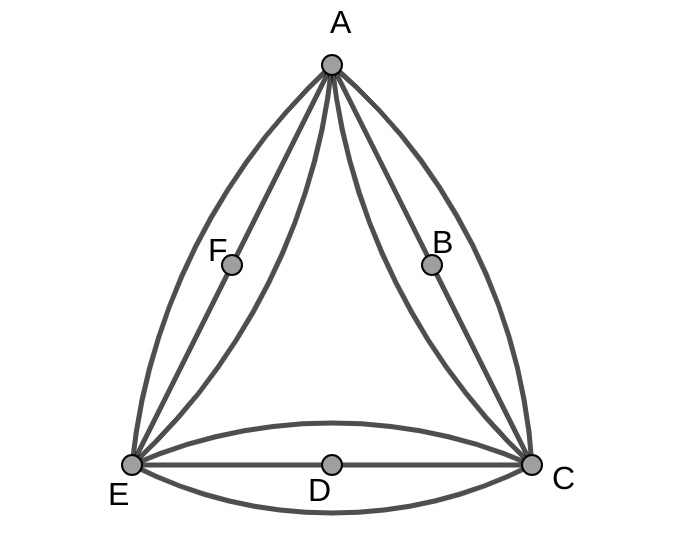
\includegraphics[width=70mm]{parallel}
  \caption{Simplicity is necessary}
  \label{fig:parallel}
\end{figure}

\begin{remark}
  Allowing triangulated disks (i.e. planar graphs with at most one face greater
  than $3$), the conjecture does not hold. For example, the graph on figure
  \ref{fig:sungraph} does not have a $2$-coupon coloring from similar reasons as
  the previous one. We will show later that this graph is a member of a bigger
  graph family without $2$ disjoint dominating sets.
\end{remark}

\begin{figure}[ht]
  \centering
  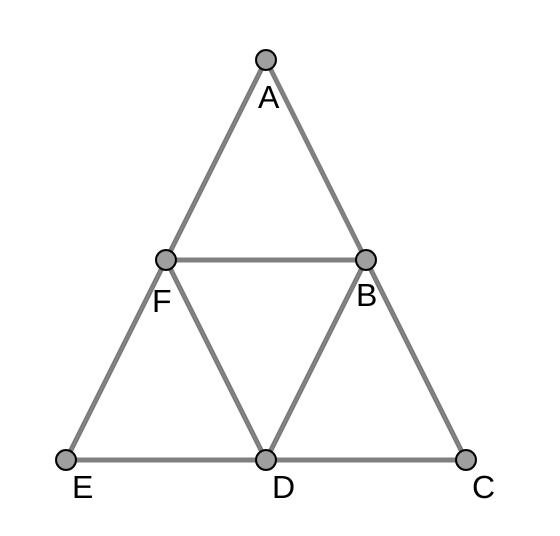
\includegraphics[width=70mm]{sungraph}
  \caption{The conjecture does not hold for triangulated disks}
  \label{fig:sungraph}
\end{figure}

\section{Fast proofs for some special cases}

There are some sufficient conditions known for having a total domatic number of
at least $2$. We will cover most of the known cases along the way. In this section
we take a look at special cases with relatively easy proofs.

The first example is a graph family for which an easy induction shows that they
are $2$-coupon colorable.

\begin{definition}
  A graph is called a stacked graph if it can be constructed from a triangle by
  repeatedly putting a new vertex in a face and connecting it with the vertices on
  the boundary of that face.
\end{definition}
\begin{remark}
  Stacked graphs are triangulated.
\end{remark}
\begin{claim}
  Stacked graphs with at least $4$ vertices are $2$-coupon colorable.
\end{claim}
\begin{proof}
  We can determine the colors of the vertices as the graph is constructed. The
  current coloring will maintain two following two properties.
  \begin{enumerate}
    \item It is a $2$-coupon coloring of the current graph.
    \item Every face has vertices from both color classes.
  \end{enumerate}
  The construction of the graph starts with a simple triangle. Color two vertices
  of the triangle to black, and the remaining vertex to white. Color the vertex added
  to the graph in the first step to white. This coloring has the desired properties.
  When a vertex is inserted into a face, color the new vertex to white, if there is
  only one white vertex on the face's boundary, and black otherwise. This trivially
  maintains the desired properties.
\end{proof}

Goddard and Henning \cite{gh} established the conjecture for some cases. We show now three
of them.

\begin{claim} \label{c:odd}
  Let $G$ be a a simple triangulated graph. If all the
  vertices of $G$ have an odd degree, then there exists a coupon coloring with $2$ colors.
\end{claim}
\begin{proof}
  There exists a proper $4$-coloring of the vertices. As every vertex $v$ has an
  odd degree, there exists an odd circle in the neighborhood of $v$. Hence, in a proper
  $4$-coloring $v$ has neighbors from at least $3$ color classes. This means that
  the union of any two color classes forms a total dominating set.
\end{proof}

\begin{claim}
  If $G$ can be obtained from a triangulated graph $H$ by putting a new vertex on every
  face and connecting them with the vertices of that face, then $G$ it $2$-coupon
  colorable.
\end{claim}
\begin{proof}
  Take a proper $4$-coloring on the vertices of $H$ and define a $2$-coloring by taking
  the union of $2-2$ color classes. The obtained coloring has the property that
  none of the faces is monochromatic. Color the added vertices to black if the face
  has only one black vertex, and color it to white otherwise.
\end{proof}

\begin{claim} \label{ham_dual}
  Let $G$ be a a simple triangulated graph of order at least $4$. If the dual
  of $G$ is Hamiltonian, then $G$ admits two disjoint total dominating sets.
\end{claim}
\begin{proof}
  Let $C$ be the Hamiltonian graph in the dual graph. Color the vertices of $G$
  inside $C$ to black, and the vertices outside of $C$ to white.
\end{proof}

\section{Variations on the conjecture}

As a reminder: the Goddard-Henning conjecture states that every simple triangulated
planar graph of order at least $4$ has total domatic number at least $2$. In this
chapter we try to find equivalent statements to the
conjecture, as well as (hopefully) slightly stronger statements. The motivation for
this chapter is that even if the stronger
statements are not true, they can be useful for proving the conjecture in special cases.

\begin{definition}
  Let $G$ be a triangulated planar graph. For a vertex $v$, each triangle
  containing $v$ has an edge not containing $v$. We call the circle consisting of
  these edges a wheel.
\end{definition}

\begin{figure}[ht]
  \centering
  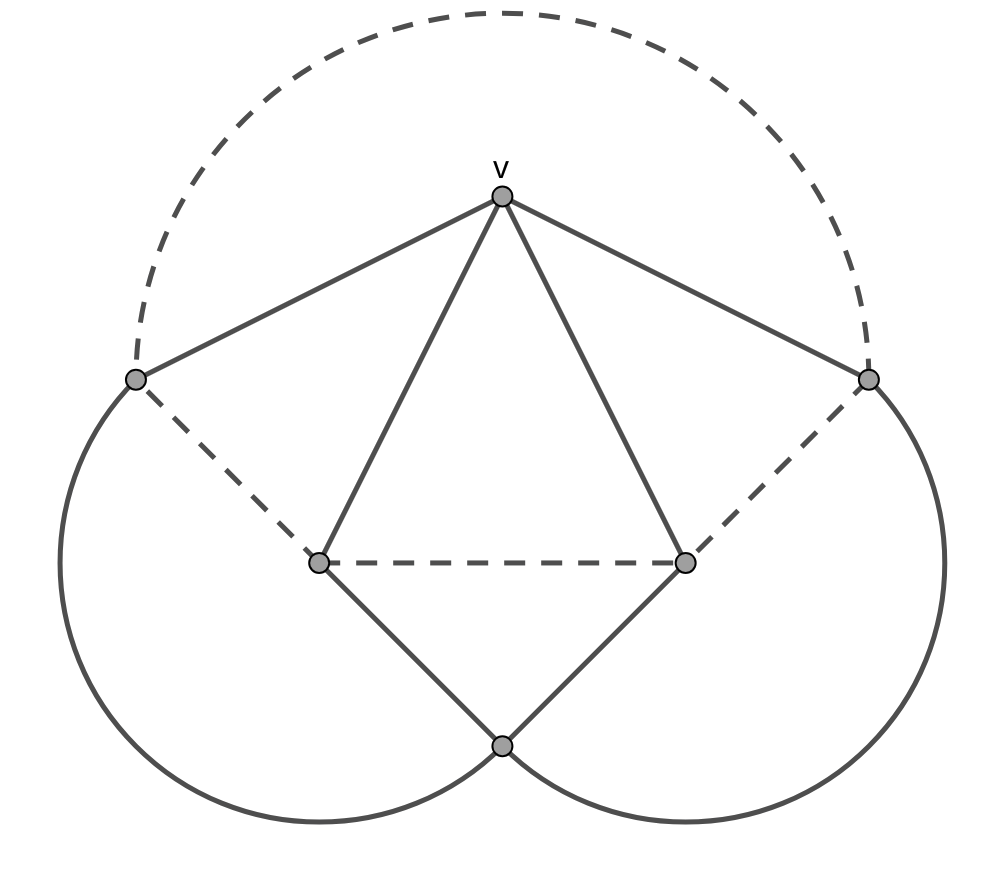
\includegraphics[width=70mm]{wheel}
  \caption{The green edges form the wheel defined by $A$ }
  \label{fig:wheel}
\end{figure}

\begin{guess}\label{s:bipartite}
  Let $G = (V, E)$ be a simple triangulated graph of order at least $4$. Then there
  exists a bipartite $H = (V, F)$ subgraph of $G$, such that $F$ contains at
  least one edge from each wheel of $G$.
\end{guess}

\begin{claim}
  The Goddard-Henning conjecture holds if and only if Statement \ref{s:bipartite} holds.
\end{claim}
\begin{proof}
  Let $G$ be a triangulated graph. Suppose first that it has a $2$-coupon coloring.
  $$F = \{uv \in E\ |\ u\ \textrm{and}\ v\ \textrm{are in different color classes}\}$$
  defines a bipartite subgraph of $G$ that contains at least one edge from each wheel.

  Now suppose that there exists bipartite subgraph that meets our requirement. Color
  the vertices in one of the classes to black, and the vertices in the other class
  to white. This is a $2$-coupon coloring of the original graph.
\end{proof}

\begin{guess}\label{s:forest}
  Let $G = (V, E)$ be a simple triangulated graph of order at least $4$. Then there
  exists a forest in $G$ containing at least one edge from each wheel.
\end{guess}

\begin{remark}
  If Statement \ref{s:forest} holds, then Statement \ref{s:bipartite} also holds.
\end{remark}

\begin{guess}\label{s:no_iso}
  Let $G = (V, E)$ be a simple triangulated graph of order at least $4$. Then there
  exists a subgraph of $H' = (V, F')$ having the following two properties.
  \begin{enumerate}
    \item $F'$ contains exactly $1$ edge from each face of $G$.
    \item There are no isolated vertices in $H'$.
  \end{enumerate}
\end{guess}

\begin{lemma}\label{l:bipartite}
  A connected planar graph is bipartite if end only if each of its faces have an
  even number of edges.
\end{lemma}
\begin{proof}
  Suppose that the graph is not bipartite and thus there exists a circle $C$ of odd
  length. We show that then exists an odd face. The proof goes by induction on the
  number of faces in the inner side of $C$. If $C$ is a face, then we are done.
  If $C$ is not a face, then there exists a face $f$ in the inner side of $C$ having at least one
  common edge with $C$. $f$ does not contain every edge of $C$, since $G$ is connected.
  Let $C'$ be the symmetric difference of the edge sets of $C$ and $f$. By the parity of $C$
  either $f$ is an odd face or $C'$ is an odd circle containing less faces in its
  inner side than $C$.

  The other direction is trivial.
\end{proof}

\begin{claim}
  Statement \ref{s:no_iso} holds if and only if Statement \ref{s:bipartite} (and thus
  the Goddard-Henning conjecture) also holds.
\end{claim}
\begin{proof}
  Let $H' = (V, F')$ be the subgraph required by Statement \ref{s:no_iso}.
  We show that $H = (V, E - F')$ is a subgraph required by Statement \ref{s:bipartite}.
  $H$ is a bipartite graph by Lemma \ref{l:bipartite}, as each of its faces have $4$ edges.
  Take a wheel $v_1v_2\dots v_k$ defined by a vertex $v$. $v$ is not an isolated vertex in $H'$, so
  there exists a vertex $v_i$ such that $vv_i \in F'$. As $F'$ contains exactly one edge
  from each face, $v_iv_{i + 1} \in F$.

  \vspace{0.4cm}

  Now let $H = (V, F)$ be the subgraph required by Statement \ref{s:bipartite}.
  Clearly, $F$ cannot contain all three edges of a face.
  We show that there exists an edge set $F_0$, such that $(V, F \cup F_0)$ is a bipartite
  subgraph of $G$ that contains exactly two edges of each face. Let $F_0 = \emptyset$.
  We will add edges to $F_0$ maintaining that $(V, F \cup F_0)$ is a bipartite graph.

  Suppose that there exists a face $uvw$ in $G$ with $uv, vw \notin F \cup F_0$, $wu \in F \cup F_0$.
  If $F \cup F_0 \cup \{ uv \}$ or $F \cup F_0 \cup \{ vw \}$ is bipartite, then
  add the appropriate edge to $F_0$. If adding either of these edges to $F_0$ creates
  an odd circle in $(V, F \cup F_0)$, then there exists a path $P_{uv}$ of odd
  length from $u$ to $v$ and a path $P_{vw}$ of odd length from $v$ to $w$. Thus $P{uv}
  + P{vw} + wu$ is a closed walk of odd length. But that is a contradiction as
  $(V, F \cup F_0)$ is a bipartite graph.

  Now suppose that there exists a face $uvw$ in $G$ such that none of its edges is
  contained in $F \cup F_0$. If either of its edges can be added to $F_0$ maintaining a
  bipartite graph, then put those edges in $F_0$. Otherwise there exist odd paths
  $P_{uv}, P_{vw}, P_{wu}$ as above. Concatenating these paths gives a closed walk
  of odd length and that yields a contradiction.

  $(V, F + F_0)$ clearly contains an edge from each wheel and contains two
  edges of each face of $G$. So $H' = (V, E - (F \cup F_0))$ contains exactly one edge
  from each face, and has no isolated vertices.
\end{proof}

One can phrase the Goddard-Henning conjecture in the dual graph as well.

\begin{claim}
  $G^* = (V^*, E^*)$ is the dual of a simple triangulated graph of order at least $4$
  if and only if $G^*$ is a $3$-regular $2$-edge-connected planar graph of order at least $4$.
\end{claim}
\begin{proof}
  It is trivial that $G^*$ is $3$-regular if and only if its dual is triangulated.

  It is also easy to see that a cut consisting of one edge corresponds to a loop
  edge in the dual, and a cut consisting of two edges corresponds to a pair of parallel edges.

  Finally, by $3$-regularity and using Euler's formula $$f^* = m^* - n^* + 2 =
  3n^*/2 - n + 2 = n^*/2 + 2,$$ where $f^*$, $m^*$, and $n^*$ denote the number of faces, edges
  and vertices of $G^*$. Thus the dual of $G^*$ has at least $4$ vertices if
  and only if $4 \le n^*/2 + 2$, i.e. $G^*$ has at least $4$ vertices.
\end{proof}

\begin{guess} \label{s:dual}
  Let $G^* = (V^*, E^*)$ be a $3$-regular $2$-edge-connected planar graph of order at least $4$.
  Then there exists a subgraph $H^* = (V^*, F^*)$ in $G^*$ that has the following $2$ properties.
  \begin{enumerate}
    \item It does not contain any odd cut of $G^*$.
    \item For every face $f$ of $G^*$, $H^*$ contains an edge $e$ not on $f$ that has at least one
    endpoint on $f$. We say that $e$ leaves the face $f$.
  \end{enumerate}
\end{guess}

\begin{claim}
  \ref{s:dual} is equivalent with \ref{s:bipartite}.
\end{claim}
\begin{proof}
  We show that given a subgraph $H = (V, F)$ that meets the requirements of \ref{s:bipartite},
  the edges corresponding to $F$ in the dual of $G$ form a subgraph $H^*$ required by
  \ref{s:dual}, and vice versa. It may be worth noting that the defined $H^*$ is
  not necessarily the same as the dual graph of $H$.

  It follows from the fact that circles of a planar graph correspond to minimal cutsets in the
  dual graph, that $H$ is bipartite if and only if $H^*$ does not contain any odd cut of $G^*$.

  Moreover, an edge from a wheel defined by $v$ in $G$, corresponds to an edge
  that leaves the face that corresponds to $v$ in the dual graph of $G$.
  Hence $H$ contains at least one edge from each wheel if and only if for every face
  of $G^*$, $H^*$ contains at least one edge that leaves that face.
\end{proof}

\begin{guess}\label{s:dual_comp}
  Let $G^* = (V^*, E^*)$ be a $3$-regular $2$-edge-connected planar graph of order at least $4$.
  Then there exists a subgraph that has the following $2$ properties.
  \begin{enumerate}
    \item It intersects every odd cut of $G^*$.
    \item For every face $f$ of $G^*$ it does not contain all the edges leaving $f$.
  \end{enumerate}
\end{guess}

\begin{claim}
  \ref{s:dual} holds if and only if \ref{s:dual_comp} holds.
\end{claim}
\begin{proof}
  If $H^*$ meets the requirements of either of the statements, the complementer subgraph in $G^*$
  meets the requirements of the other.
\end{proof}

A $2$-factor of a graph $G = (V, E)$ consists of disjoint circles covering $V$.
We can formulate a sufficient condition for the Goddard-Henning conjecture with
the help of $2$-factors. The motivation for such a reformulation is the fact that
the existence of $2$-factors in which some cycles are not allowed, is a well-studied
part of graph theory.

\begin{guess} \label{s:2-factor}
  Let $G^* = (V^*, E^*)$ be a $3$-regular $2$-edge-connected planar graph of order at least $4$.
  Then there exists a $2$-factor not containing any of the faces.
\end{guess}
\begin{claim} \label{c:2-factor}
  If Statement \ref{s:2-factor} holds, then \ref{s:dual} holds.
\end{claim}
\begin{proof}
  Let $H^* = (V^*, F^*)$ be the $2$-factor containing none of the faces of $G^*$.

  Every cut of $G^*$ has an even number of common edges with every circle in $H^*$.
  Therefore $H^*$ does not contain any odd cuts of $G^*$.

  Let $f = v_1v_2 \dots v_l$ be a face of $G^*$. As $F^*$ does not contain $f$,
  there must exist a $v_i$ such that $v_iv_{i + 1} \notin F^*$. Moreover, every
  vertex has degree $2$ in $H^*$, so there is an edge starting from $v_i$ that leaves $f$.
\end{proof}

Statement \ref{s:2-factor} can easily be converted into a statement about perfect matchings.

\begin{guess} \label{s:matching}
  Let $G^* = (V^*, E^*)$ be a $3$-regular $2$-edge-connected planar graph of order at least $4$.
  Then there exists a perfect matching containing at least one edge from each face.
\end{guess}
\begin{claim}
  Statement \ref{s:2-factor} holds if and if Statement \ref{s:matching} holds.
\end{claim}
\begin{proof}
  As $G^*$ is $3$-regular, a subgraph is a $2$-factor if and only if the complementer
  subgraph is a perfect matching. Clearly, a subgraph contains none of the faces
  if and only if the complementer subgraph does contain at least one edge from
  each face.
\end{proof}

TODO: Add a figure about these statements.


\chapter{Proofs for special cases of the Goddard-Henning conjecture} \label{ch:spec}
\section{Outerplanar and Hamiltonian graphs}
Zoltán Lóránt Nagy \cite{outerplanar} showed that the conjecture of Goddard and Henning holds for
Hamiltonian graphs. For this, he characterized the $2$-coupon colorable
maximal outerplanar graphs first.

\begin{definition}
   A graph is outerplanar if it has a planar drawing for which all vertices
   belong to the outer face. A maximal outerplanar graph is a simple outerplanar graph
   such that adding any edge results in a non-outerplanar graph.
\end{definition}
\begin{remark}
  The outer face of a maximal outerplanar graph is a Hamiltonian cycle.
\end{remark}

In order to provide the mentioned characterization we need to introduce a few
notions first.
\begin{definition}
  Let $G$ be a maximal outerplanar graph of order $n \ge 3$. The $M(G)$ sun graph
  of $G$ is obtained by gluing a triangle to each edge of the outer face.
\end{definition}
\begin{remark}
  $M(G)$ is a maximal outerplanar graph with $2n$ vertices, from which $n$ has
  degree $2$.
\end{remark}
\begin{remark}
  If $G$ has an odd number of vertices, then $M(G)$ does not have two disjoint
  total dominating sets, as in a $2$-coupon coloring of $M(G)$ the vertices of
  $G$ must have alternating colors. The graph on figure $\ref{fig:sungraph}$ is
  the sun graph of the $BDE$ triangle.
\end{remark}
\begin{definition}
  A vertex $v$ of a maximal outerplanar graph is called a central vertex if the
  following $3$ conditions hold.
  \begin{enumerate}
    \item $deg(v) \ge 3$
    \item Every neighbor of $v$ has degree at least $3$.
    \item For every $u, w$ neighbors of $v$ the length of the $uw$ path on the
    outer face not containing $v$ is divisible by $4$.
  \end{enumerate}
\end{definition}
\begin{claim}
  The outer face of a maximal outerplanar graph does not contain two consecutive
  central vertices.
\end{claim}
\begin{proof}
  Suppose there exists an $uv$ edge on the outer face such that $u$ and $v$ are
  central vertices. Because of the maximality of the graph there exists a $uvw$
  triangle. Index the vertices along the outer face form $v = v_1$ to $u = v_{n}$.
  Suppose $w = v_i$. From the centrality of $v$ follows that $i \equiv 2\
  (\textrm{mod}\ 4)$. On the other hand, $u$ is also a central vertex, hence
  $i \equiv 1\ (\textrm{mod}\ 4)$.
\end{proof}
\begin{definition}
  A generalized sun graph is a maximal outerplanar graph of order
  $n \equiv 2\ (\textrm{mod}\ 4)$ such that the number of
  degree $2$ vertices plus the number of central vertices is $n/2$.
\end{definition}
\begin{remark}
  Every second vertex of the outer face in a generalized sun graph is either
  central or has degree $2$.
\end{remark}

The key characterization theorem is the following.

\begin{thm}\label{thm:outerplanar}
  Let $G$ be a maximal outerplanar graph of order at least $4$. $G$ admits $2$ disjoint total dominating
  sets if and only if $G$ is not a generalized sun graph.
\end{thm}

For proving this theorem we need some observations about generalized sun graphs.

\begin{definition}
  Let $G$ be a maximal outerplanar graph and $i \ge 2$. We say that a $uv$ edge is a chord
  of length $i$, if there is a $uv$ path of length $i$ on the outer face. (This means
  that if $uv$ is a chord of length $i$, then it is also a chord of length $n - i$.)
\end{definition}

\begin{lemma} \label{lem:two_chord}
  A maximal outerplanar graph of order $n \ge 3$ has a chord of length $2$.
\end{lemma}
\begin{proof}
  It is trivial for $n = 3$. Suppose $n \ge 4$ and
  let $uv$ be a chord of minimal length. By
  the maximality of the graph there exists a $uvw$ face, where $w$ is on the shorter
  $uv$ path of the outer face. If $uv$ is not a chord of length $2$, then $uw$ or $vw$
  is a chord of length less than the length of the $uv$ chord.
\end{proof}

\begin{lemma} \label{lem:3-4_chord}
  A maximal outerplanar graph of order $n \ge 5$ has a chord of length $3$ or $4$.
\end{lemma}
\begin{proof}
  Let $uv$ be a chord of minimal length among chords of length at least $3$. By
  the maximality of the graph there exists a $uvw$ face, where $w$ is on the $uv$ path
  on the outer face that defines the length of the chord. If on this path $w$ has a distance
  bigger than $2$ from either $u$ or $v$, than $uw$ or $vw$ is a chord contradicting
  the minimality of $uv$. Thus, the length of the $uv$ path is at most $4$.
\end{proof}

\begin{lemma} \label{lem:del_face}
  If $G$ is a maximal planar graph of order $n \ge 7$, then there exists a bounded
  face, such that the deletion of this face divides $G$ into three graphs with the
  following properties.
  \begin{enumerate}
    \item At most one of the three graphs has more than $3$ bounded faces.
    \item At least one of the three graphs has $2$ or $3$ faces.
  \end{enumerate}
\end{lemma}
\begin{proof}
  For $n \le 11$, the statement is easy to verify.

  For $n > 11$ delete the faces with $2$ common edges with the unbounded face. Then in the remaining
  graph $G_1$ delete the faces that now have $2$ common edges with the unbounded face.

  We claim that the remaining graph $G_2$ is not empty. $G$
  has $m = \frac{3(f - 1) + n}{2}$ edges, where $f$ denotes the number of faces.
  Then by Euler's formula $n = f + 1$, hence $G$ has at least $11$ faces. In the
  first deleting step at most $n/2$ faces are deleted, and in the second step at most
  $|G_1|/2$ faces are deleted. Thus at most $3(f + 1) / 4$ faces are deleted.
  $3(f + 1) / 4 \le f - 2$ if $f \ge 11$.

  Finally, choose a face $f_0$ from the remaining graph $G_2$, that has $2$ common edges with
  the unbounded face of $G_2$. We claim that $f_0$ has the desired properties. $f_0$ has at most
  one neighboring face in $G_2$, and one or two neighboring faces $f_1$ and maybe $f_2$ outside of $G_2$.
  Both of $f_1$ and $f_2$ has at most two neighboring faces outside of $G_1$, and
  at least one of $f_1$ and $f_2$ has at least one neighboring face outside of $G_1$.
\end{proof}

\begin{proof}[Proof of Theorem \ref{thm:outerplanar}]
  First we show that generalized sun graphs do not have $2$ disjoint total
  dominating sets. The proof goes by induction on the $n = 4k + 2$ number of vertices.

  For $k = 1$ there is only one generalized sun graph and it does not admit $2$
  disjoint total dominating sets. (Shown on figure \ref{fig:sungraph}.)

  Suppose $k \ge 2$ and $G$ is a generalized sun graph of order $4k + 2$. Index
  the vertices along the outer face from $v_1$ to $v_{4k + 2}$, such that every
  vertex with an odd index is central or has degree $2$. Let $c$ be a $2$-coloring of
  the graph. We show that $c$ cannot be a $2$-coupon coloring. The cardinality of the
  vertices implies that there must be two consecutive vertices $v_{2i}$ and $v_{2i + 2}$
  with the same color (say white). If $v_{2i + 1}$ has only white neighbors, then this
  coloring is not a $2$-coupon coloring. So suppose $v_{2i + 1}$ has a black neighbor
  $v_j$. In this case $v_{2i + 1}$ is a central vertex. The $v_{2i + 1}v_j$ edge divides the graph
  into two parts ($v_{2i + 1}v_j$ is an edge in both graphs). Both of
  these graphs are generalized sun graphs, as $v_{2i + 1}$ either remains a central
  vertex or becomes a vertex of degree $2$ in these smaller graphs, whereas other
  central vertices remain central vertices. By induction, the restriction of
  $c$ is not a $2$-coupon coloring in either of the smaller graphs. If there is
  a vertex $v_l$ with a monochromatic neighborhood in one of the smaller graphs
  and $l \neq 2i + 1,\ l \neq j$, then $v_l$ has the same neighborhood in $G$, hence
  all its neighbors are from the same color class. $v_{2i + 1}$ cannot violate the
  condition, as it was chosen in a way that it has both a black and a white neighbor
  in both graphs. Thus the only remaining case is when $v_j$ has a monochromatic
  neighborhood in both graphs. But in this case all of its neighbors are from
  the same color class as $v_{2i + 1}$, so it has a monochromatic neighborhood also
  in $G$.

  \vspace{0.4cm}

  Now we show that if a graph $G$ of order $n$ is not a generalized sun graph
  then it does have two disjoint total dominating sets.

  If $n \equiv 0\ (\textrm{mod}\ 4)$, then it is easy to find a $2$-coupon coloring:
  color the vertices along the boundary of the outer face by repeating the pattern
  $BBWW$.

  If $n \equiv 1\ (\textrm{mod}\ 4)$, then the same coloring method works, if you
  start the coloring from the right vertex. By lemma \ref{lem:two_chord} there
  exists a chord $uv$ of length $2$. Alternating colors in pairs starting from $v$
  does the job. (See Figure \ref{fig:4k+1}.)
  \begin{figure}[h]
    \centering
    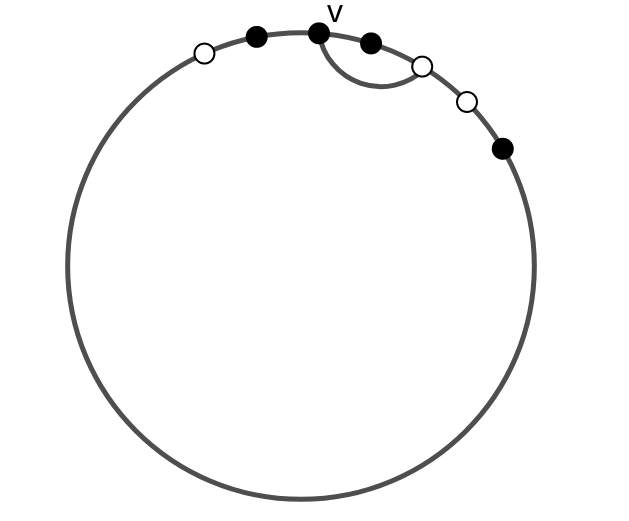
\includegraphics[width=50mm]{4k+1}
    \caption{Coloring an outerplanar graph of order $4k + 1$}
    \label{fig:4k+1}
  \end{figure}

  If $n \equiv 3\ (\textrm{mod}\ 4)$, then start the coloring from a vertex next
  to $v$. (See Figure \ref{fig:4k+3}.)
  \begin{figure}[h]
    \centering
    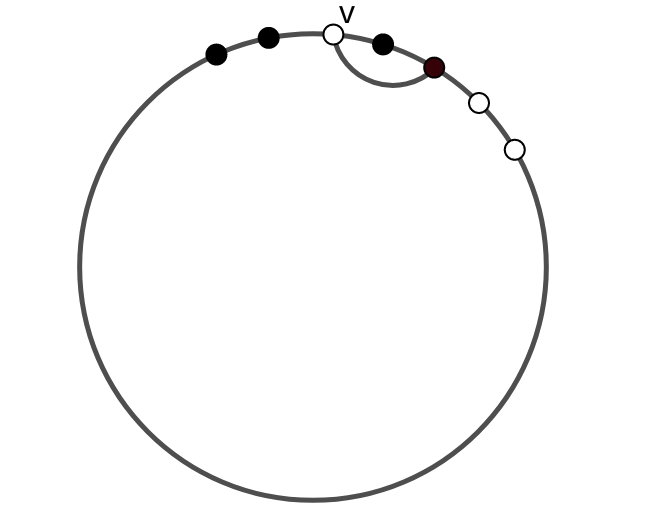
\includegraphics[width=50mm]{4k+3}
    \caption{Coloring an outerplanar graph of order $4k + 3$}
    \label{fig:4k+3}
  \end{figure}

  Suppose $n \equiv 2\ (\textrm{mod}\ 4)$. We show by induction that if $G$ does not have $2$
  disjoint total dominating sets, then it is a generalized sun graph.\\
  The case $k = 1$ is easy to check.\\
  If $G$ has a chord $uv$ of length $3$, then $uv$ divides the graph into two parts:
  $G_1$ of order $4$ and $G_2$ of order $4k$. By alternating colors in pairs one can obtain
  $2$-coupon colorings of $G_1$ and $G_2$, where both $u$ and $v$ are colored to black
  in both graphs.\\
  If $G$ does not have a chord of length $3$, then by Lemma \ref{lem:3-4_chord}
  there exists a chord $uv$ of length $4$. Then $uv$ divides $G$ into two graphs.
  One of them must be the maximal outerplanar graph $G_5$ of order $5$. $u$ and $v$
  must be the degree $3$ vertices of $G_5$, as otherwise there would be a chord of length $3$
  in $G$. Note that in a $2$-coupon coloring $u$ and $v$ must have the same colors
  in order to create a proper neighborhood for the degree $2$ vertices of $G_5$.
  Consider the face $uvw$, where $w$ is not in $G_5$. The deletion of this face
  divides $G$ into $3$ graphs: $G'$, $G''$ and $G_5$. (It might be that $G'$ or $G''$ is
  degenerated in the sense that it consists only of one edge.) Let $G'$ be the graph containing
  $u$ and $w$. Without loss of generality we may assume that $|G''| \le |G'|$.\\
  Choose the $uv$ chord in a way, such that $|G'|$ is minimal. We may assume that
  $G'$ has at most $3$ faces by Lemma \ref{lem:del_face}, and thus $|G'| \le 5$.
  Thus, there are $4$ cases depending on the size of $G'$.

  \begin{itemize}
    \item Case $1$: $|G'| = 2$.
      In this case $G''| = 4k - 2$. If $G''$ has a $2$-coupon coloring, then
      it can easily be expanded to a $2$-coupon coloring of $G$. If $G''$ does
      not have a $2$-coupon coloring, then it is a generalized sun graph by induction.
      If $v$ is a degree $2$ or central vertex in $G''$, then color the vertices of $G''$ by
      alternating colors in pairs, starting with white from $w$, but color $v$ to
      black. Let $x$ denote the vertex before $v$. (See Figure \ref{fig:case1}.)
      \begin{figure}[h]
        \centering
        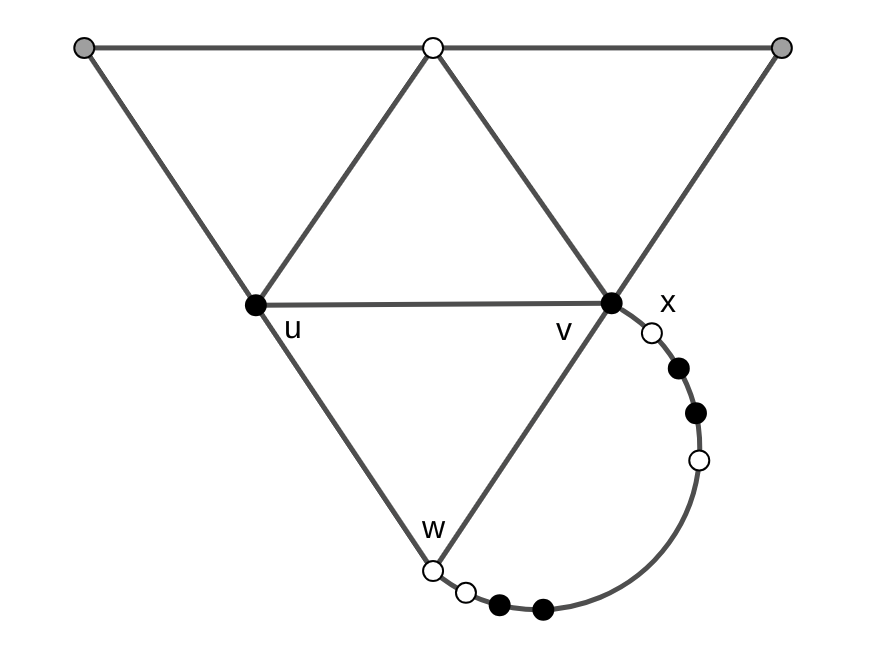
\includegraphics[width=60mm]{case1}
        \caption{Case $1$}
        \label{fig:case1}
      \end{figure}
      This way, only $v$ can have a monochromatic neighborhood in $G''$: if $v$ has degree
      $2$, then $wx$ is an edge, and if $v$ is central, then $v$ and $x$ have a common
      neighbor in $G''$ and $v$ has only white neighbors. $G_5$ can be colored to
      provide $v$ the missing color. \\

      If $v$ is neither a degree $2$ vertex nor a central vertex, then $w$ is. In
      this case $w$ is a central vertex in $G$ and thus $G$ is a generalized sun graph.
    \item Case 2: $|G'| = 3$.
      In a $2$-coupon coloring $u$ and $v$ must have the same color, whereas $u$
      and $w$ must have different colors. Let $H$ be the graph obtained from $G$
      by deleting $G_5$ and identifying $uw$ with $vw$. (See \ref{fig:case2})
      $G$ is $2$-coupon colorable if and only if $H$ is $2$-coupon colorable. On the other hand,
      $G$ is a generalized sun graph if and only if $H$ is a generalized sun graph.
      \begin{figure}[h]
        \centering
        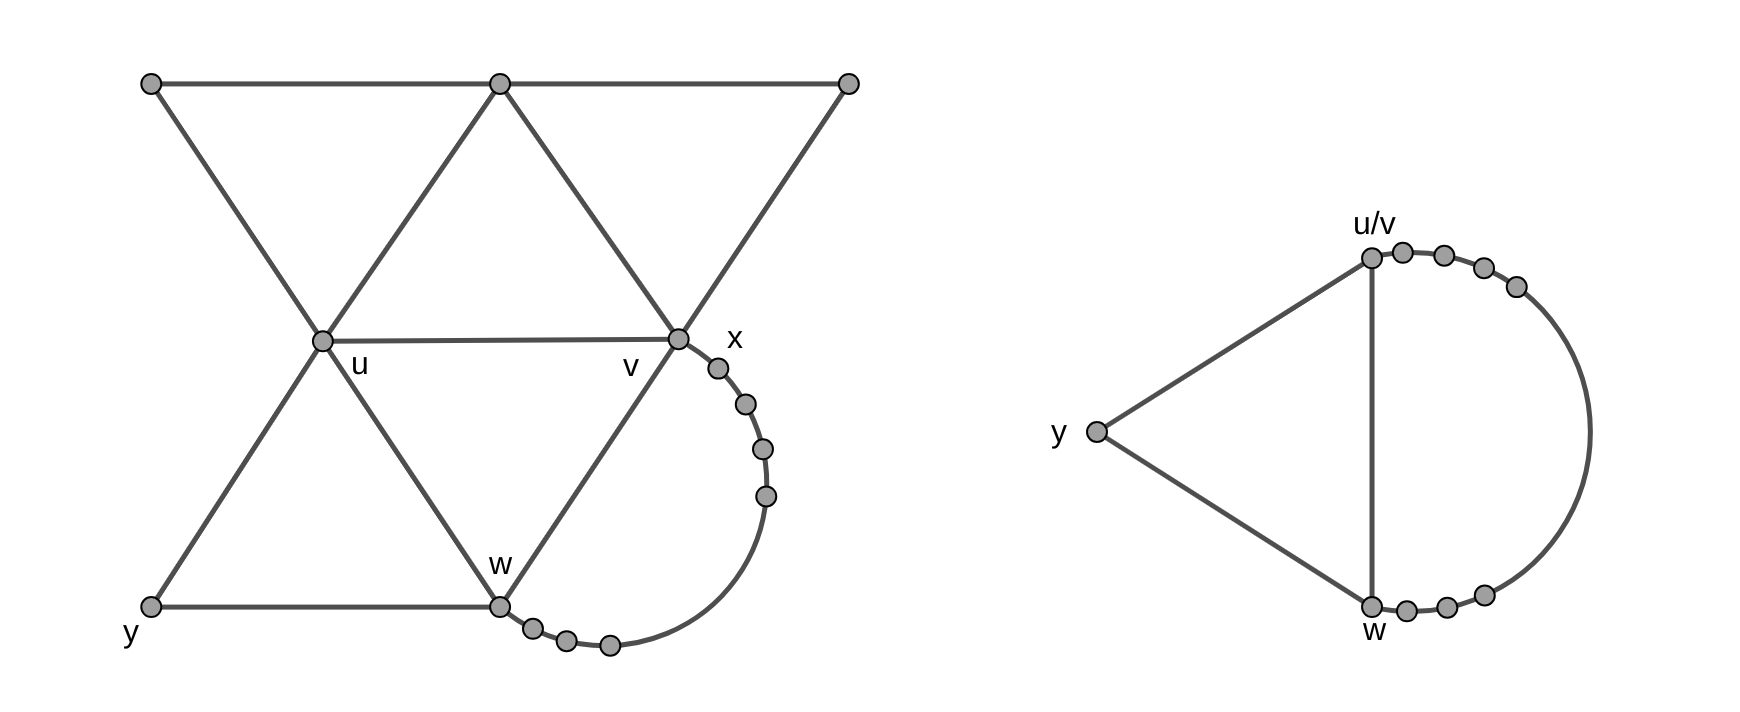
\includegraphics[width=150mm]{case2}
        \caption{Case $2$: $G$ (left) and $H$ (right)}
        \label{fig:case2}
      \end{figure}
    \item Case $3$: $|G'| = 4$.
      If $|G'| = 4$, then $uw$ is a chord of length $3$, and that is a contradiction.
    \item Case $4$: $|G'| = 5$.
      $u$ and $w$ must be the degree $3$ vertices in $G'$, otherwise we could
      find a chord of length $3$. In a $2$-coupon coloring $u$ and $w$ must have
      the same color. Let $H$ be the graph obtained from $G$ by deleting $G_5$
      and identifying $uw$ with $vw$. (See \ref{fig:case4})
      \begin{figure}[h]
        \centering
        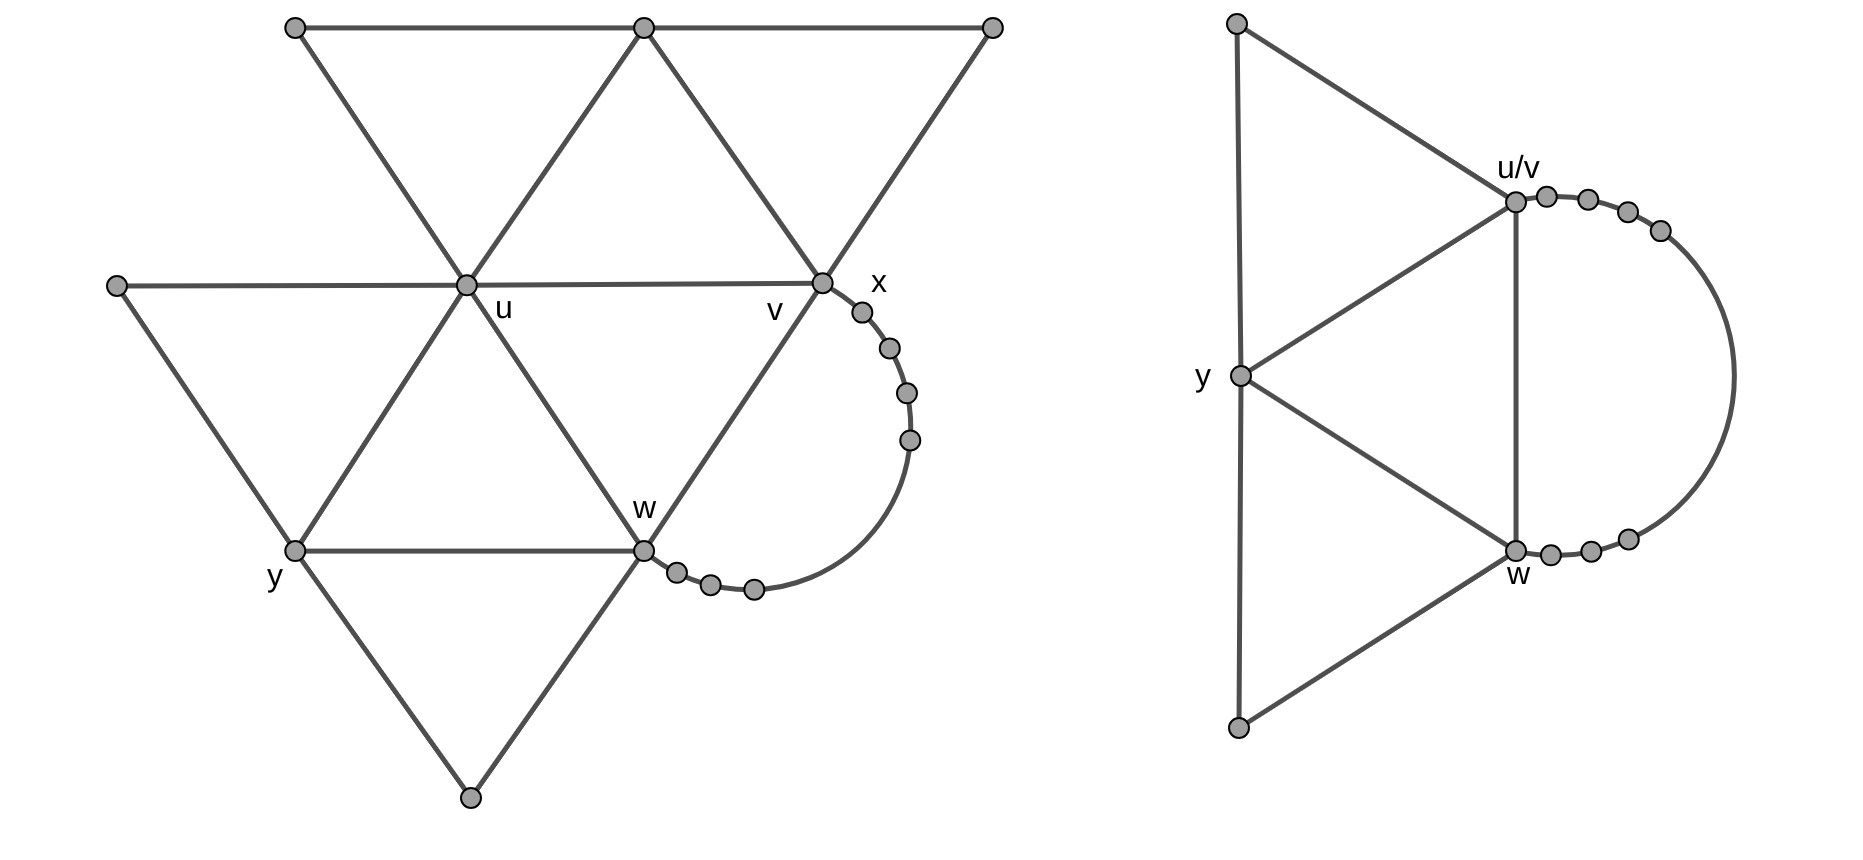
\includegraphics[width=150mm]{case4}
        \caption{Case $4$: $G$ (left) and $H$ (right)}
        \label{fig:case4}
      \end{figure}
      $G$ is $2$-coupon colorable if and only if $H$ is $2$-coupon colorable. On the other hand,
      $G$ is a generalized sun graph if and only if $H$ is a generalized sun graph.
  \end{itemize}
\end{proof}

\begin{remark}
  With a slight modification of the proof it can be shown that the vertices of a
  generalized sun graph cannot be colored in a way that every degree $2$ or central
  vertex has neighbors from both color classes.
\end{remark}

As mentioned earlier, based on this theorem Zoltán Lóránt Nagy \cite{outerplanar}
also showed that the total dominating number of Hamiltonian triangulated graphs
is at least two. We still need a Lemma for proceeding with the proof.

\begin{lemma}\label{lem:central}
  If $G$ is a generalized sun graph of order $4k + 2$, then there exist at most
  $k - 1$ chords incident to a central vertex.
\end{lemma}
\begin{proof}
  The proof goes by induction. If $k = 1$, then there exists only one generalized sun graph
  of order $4k + 2$, and it does not have any central vertices. Suppose $k > 1$.
  We are done, if there is no chord incident to a central vertex. Otherwise, let $uv$ be
  such a chord of minimal length, where $v$ is central. $uv$ divides the graph into
  two generalized sun graphs. In both of these graphs, $v$ is either a degree $2$
  vertex or a central vertex. Hence all the chords incident to a central vertex in $G$
  must be either $uv$ or a chord with the same property in one of the smaller graphs.
  By the minimality of $uv$, one of these graphs does not have chords incident to
  a central vertex. The other graph is of order at most $4(k - 1) + 2$, thus by induction
  it contains at most $k - 2$ chords incident to a central vertex.
\end{proof}

\begin{cor} \label{col:degree2}
  In a generalized sun graph the number of central vertices is less than the number
  of degree $2$ vertices.
\end{cor}
\begin{proof}
  Let $G$ be a generalized sun graph of order $4k + 2$. The number of central
  vertices is at most $k - 1$ by the previous lemma. The number of degree $2$ or
  central vertices is $2k + 1$.
\end{proof}

\begin{thm} \label{thm:ham}
  Every triangulated graph with a Hamiltonian circle admits $2$ disjoint
  dominating sets.
\end{thm}
\begin{proof}
  A Hamiltonian triangulated graph $G$ can be obtained by identifying the Hamiltonian cycle
  of two maximal outerplanar graphs $G_1$ and $G_2$. If at least one of these outerplanar graphs is
  $2$-coupon colorable, then the same coloring is a $2$-coupon coloring of $G$.
  By Theorem \ref{thm:outerplanar} we are done if at least one of these graphs is
  not a generalized sun graph.

  Suppose that $G_1$ and $G_2$ are generalized sun graphs. If the union of degree
  $2$ vertices and central vertices is the same in $G_1$ and $G_2$, then by Corollary
  \ref{col:degree2} there exists a vertex with degree $2$ in both graphs. Then this
  vertex is a degree $2$ vertex in $G$ and that is a contradiction, as in a triangulated
  planar graph every degree must be at least $3$.

  Assume that each vertex is a degree $2$ or central vertex in $G_1$ or $G_2$.
  Index the vertices along the Hamiltonian cycle from $v_1$ to $v_{4k + 2}$.
  We claim that there exists an index $i$ such that $v_i$ is a degree $2$ vertex
  in $G_1$ and $v_{i + 3}$ is a degree $2$ vertex in $G_2$. (If $i + 3$ is bigger than
  $4k + 2$, we take $v_{i + 3 - (4k + 2)}$.) Let $I_1 = \{i | deg_{G_1}(v_i) = 2\}$,
  $I_2 = \{i | deg_{G_2}(v_i) = 2\}$ and $J = \{i + 3 | i \in I_1\}$. By Corollary
  \ref{col:degree2} the cardinality of all of these sets is at least $k + 2$, hence
  there exists an index $i$ such that $i + 3 \in I_2 \cap J$, proving the claim.

  Finally, we define a $2$-coupon coloring of $G$ as follows. Let $v_i$ be a vertex
  as above. Color the vertices by alternating colors in pairs starting from $v_{i + 2}$.
  (See Figure \ref{fig:ham}.) It is clear that all the vertices apart from $v_{i + 1}$
  and $v_{i + 2}$ have neighbors in both color classes. However, $v_i$ is a degree $2$ vertex
  in $G_1$, hence $v_{i - 1}v_{i + 1}$ is an edge in $G_1$. Similarly, $v_{i + 2}v_{i + 4}$
  is an edge in $G_2$. These two edges ensure that $v_{i + 1}$ and $v_{i + 2}$ also
  have neighbors in both color classes.
  \begin{figure}[h]
    \centering
    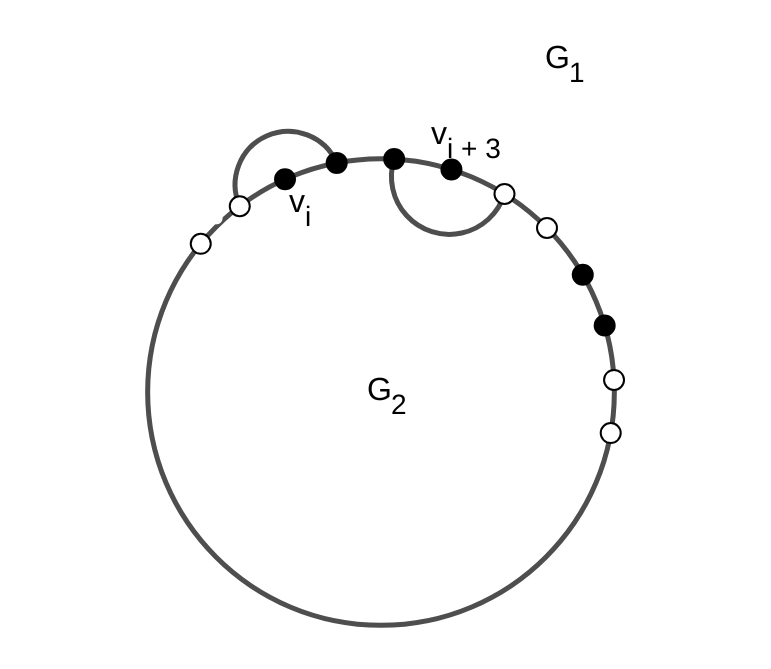
\includegraphics[width=60mm]{hamilton}
    \caption{Coloring a Hamiltonian graph}
    \label{fig:ham}
  \end{figure}
\end{proof}

\begin{remark}
  Whitney \cite{ham1} proved that each triangulated planar graph without separating
  triangles is Hamiltonian. Helden \cite{ham5} strengthened this statement by proving that
  each triangulated planar graph with at most five separating triangles is Hamiltonian.
\end{remark}

With the help of these theorems,
we can also say something about graphs with another kind of $2$-factors.

\begin{claim}
  Let $G$ be a simple triangulated graph of order $n \ge 4$. If $G$ has a $2$-factor
  with none of its cycles having length congruent to $2$ modulo $4$, then the total
  dominating number of $G$ is at least $2$.
\end{claim}

\begin{proof}
  If the $2$-factor consists only of one cycle, then Theorem \ref{thm:ham} proves the
  claim. Suppose that there are at least two cycles in the $2$-factor. First note that
  by alternating colors in pairs, any cycle of length not congruent to $2$ modulo $4$
  can be colored in a way, such that there is at most one vertex with a monochromatic neighborhood.
  (See Figures \ref{fig:4k+1}, \ref{fig:4k+3}.)

  Contract each cycle to a single vertex. $G$ is connected, hence there exists a tree $T$
  in the contracted graph. Choose $T$ to have a minimal number of degree $1$ vertices.
  Let $E(T)$ denote the edges of the original graph that were mapped
  to $T$. We show a $2$-coupon coloring in the subgraph defined by the union of the $2$-factor
  and $E(T)$. Choose a root node $r$ from the degree $1$ vertices in $T$.

  We color the cycle $C_0$
  corresponding to $r$ first. Choose a vertex $v$ in $C_0$, such that there exists a
  $uv$ edge in $E(T)$. We color $C_0$ such that only $v$ may have a monochromatic
  neighborhood and assign $u$ the missing color.

  After this, we iteratively
  color a child of a cycle that is already colored.
  We start by coloring cycles that do not
  correspond to leaves in $T$. Suppose that $C_1$ is a cycle like that, let $C_2$
  be a child of $C_1$, and $v_1v_2$
  be the edge in $E(T)$ such that $v_1 \in C_1$ and $v_2 \in C_2$. Let $c_1$ be a coloring of
  $C_1$ such that only $v_1$ may have a monochromatic neighborhood. There might be
  a vertex (but only one) in $C_1$ that already has a color, so flip the colors of $c_1$ if
  necessary. Color $v_2$ in a way that provides $v_1$ the missing color.

  Now we
  color cycles that correspond to leaves, but have at least $4$ vertices. Let $C_l$ be a
  cycle like that. By Theorem \ref{thm:outerplanar} there
  exists a $2$-coupon coloring $c_l$ of $C_l$. Again, if there is a vertex in $C_l$ that
  already has a color, then we might need to flip the colors of $c_l$.

  Finally, we need to
  color cycles corresponding to leaves of $T$ and having only $3$ vertices. Let $u_lv_lw_l$ be
  a cycle like that, where $v_l$ is the only vertex that may already have a color. Suppose it
  is colored to black. There exists a face $v_lw_lx_l$ where $x_l \neq u_l$.
  If $x_l$ is colored to black, then color $w_l$ and $u_l$ to white. If $x_l$ is colored
  to white, then color $w_l$ to white, and $u_l$ to black. The only remaining case is
  when $x_l$ does not have a color yet. In this case, there must be a face $x_ly_lz_l$
  corresponding to a leaf of $T$. These two leaves have a closest common ancestor
  $t$. $t$ is of degree at least $2$ in $T$, hence $t \neq r$, so $t$ must have degree
  at least $3$. By adding the edge corresponding to $v_lx_l$ to $T$ and removing
  the first edge of the $tv_l$ path, we would get a tree $T'$, where $T'$ would have
  fewer degree $1$ vertices then $T$ has. This contradicts to the choice of $T$.
\end{proof}

\section{Graphs without low-degree vertices}
With the help of hypergraphs, we TODO

\begin{definition}
  Let $H$ be a hypergraph. The incidence graph of $H$ is a bipartite graph with one of
  its classes corresponding to the vertices of $H$, and the other class corresponding to
  the hyperedges of $H$. $ve$ is an edge in the incidence graph if and only if the
  hyperedge $e$ contains vertex $v$ in $H$.
\end{definition}
\begin{definition}
  A hypergraph is called planar, if its incidence graph is planar.
\end{definition}
\begin{definition}
  A vertex coloring of a hypergraph is proper if all its hyperedges contain vertices
  from both color classes.
\end{definition}

\begin{thm} \label{thm:hyper}
  Let $H = (V, E)$ be a planar hypergraph with at most $2$ hyperedges of size $2$. Then $H$ has
  a proper vertex coloring with two colors.
\end{thm}
\begin{proof}
  We may assume that $H$ has exactly $2$ hyperedges of size $2$. Otherwise add
  one or two new hyperedges of size $2$. A proper coloring of the resulting hypergraph
  is also a proper coloring of the original one.

  We define another planar graph based on the incidence graph of $H$ as follows.
  For each hyperedge $e$, delete the corresponding vertex from the graph, and
  add edges between the vertices contained in $e$ in a way that it results in a circle.
  The bounded faces of the resulting graph $G_H=(V, F)$ correspond to the hyperedges of $H$.
  (See Figure \ref{fig:hyper}.) After this, triangulate the faces that have more than
  $3$ vertices.

  \begin{figure}[h]
    \centering
    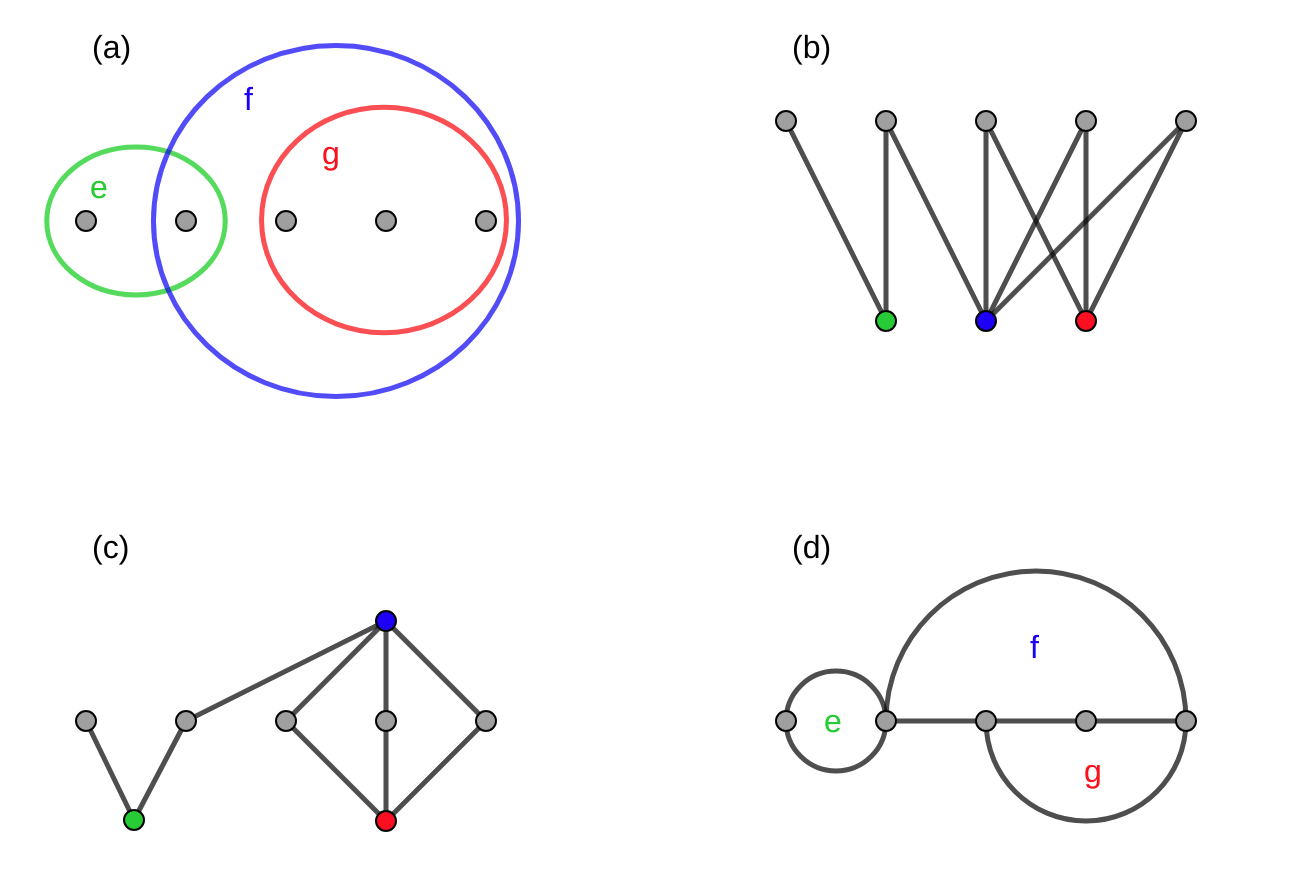
\includegraphics[width=150mm]{hypergraph}
    \caption{A hypergraph (a), its incidence graph (b), a planar embedding of the
      incidence graph (c) and the graph $G_H$ (d)}
    \label{fig:hyper}
  \end{figure}

  Let $c_4$ be a proper $4$-coloring of the resulting graph with colors $\{1, 2, 3, 4\}$.
  By permuting the color classes if necessary, we may assume the followings.
  \begin{enumerate}
    \item If the two hyperedges of size $2$ are not disjoint, i.e. they are $\{u, v\}$ and
      $\{u, w\}$, then $c_4(u) 1$, and $c_4(v), c_4(w) \in \{3, 4\}$.
    \item If the two hyperedges of size $2$ are disjoint, i.e. they are $\{u, v\}$ and
      $\{x, y\}$, then $c_4(u), c_4(x) \in \{1, 2\}$ and $c_4(v), c_4(y) \in \{3, 4\}$.
  \end{enumerate}
  We define a $2$-coloring of $G_H$ as follows.
  \[
    c_2(v) = \begin{cases}
      1, & \text{if}\ c_4(v) = 1 \ \text{or}\ c_4(v) = 2\\
      2, & \text{if}\ c_4(v) = 3 \ \text{or}\ c_4(v) = 4\\
    \end{cases}
  \]
  We claim that $c_2$ is a proper $2$-coloring of $H$. The hyperedges of size $2$
  have vertices in both color classes due to our assumptions on $c_4$. For the other
  hyperedges there exists a face in $G$ containing the vertices of the hyperedge.
  As $c_4$ was a proper $4$-coloring of the triangulated graph, each face of $G$
  of size at least $3$ has vertices from $3$ or $4$ color classes.
\end{proof}

\begin{claim}
  Let $G$ be a simple triangulated graph. If there are at most two vertices of degree
  at most $4$, then $G$ has a $2$-coupon coloring.
\end{claim}
\begin{proof}
  By Claim \ref{c:dual} the dual $G^*$ is a $3$-regular $2$-edge-connected planar graph.
  Thus, by Petersen's theorem there exists a perfect matching $M$ in $G^*$. By deleting
  the edges corresponding to $M$ from $G$, we get a graph $G'$ such that all its faces contains
  $4$ vertices. We call such graphs quadrangulated. Note, that for each vertex $v$,
  we deleted at most the half of the vertices starting from $v$, thus there are at most
  two vertices in $G'$ of degree $2$ and none of the vertices has less than $2$ neighbors.

  By Lemma \ref{l:bipartite}, $G'$
  is a bipartite graph. Let $U$ and $V$ be the two classes of $G'$. $G'$ is the incidence
  graph of two hypergraphs: let $H_1$ be the hypergraph defined on the vertex set
  $U$ with hyperedges $V$, and $H_2$ be the hypergraph defined on the vertex set $V$
  with hyperedges $U$. By Theorem \ref{thm:hyper} $H_1$ and $H_2$ has proper $2$-colorings.
  Take the union of these colorings $c$. I.e. on the vertices of $U$, $c$ is defined
  by a proper coloring of $H_1$, whereas on the vertices of $V$, $c$ is defined
  by a proper coloring of $H_2$. $c$ is a $2$-coupon coloring of $G'$.
\end{proof}

\begin{remark}
  It is not true that every simple quadrangulated graph has a $2$-coupon coloring.
  See Figure \ref{fig:quad} for an example.
\end{remark}
\begin{figure}[h]
  \centering
  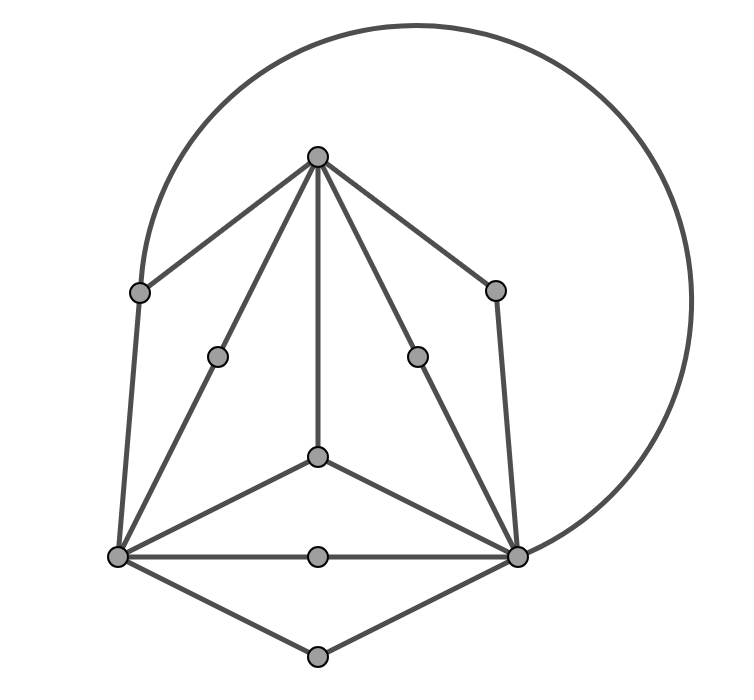
\includegraphics[width=60mm]{quad}
  \caption{A quadrangulated graph without two disjoint dominating sets}
  \label{fig:quad}
\end{figure}

\begin{conj}
  If $G$ is a simple triangulated graph with all the vertices of degree at least
  $4$, then $G$ admits three disjoint total dominating sets.
\end{conj}


It is also worth noting that having total dominating number at least $2$ can be
translated into a statement about the so-called neighborhood hypergraph. The neighborhood
hypergraph of $G$ is a hypergraph defined on the vertex set of $G$, where for each vertex
$v$, there is a hyperedge containing the neighboring vertices of $v$. $G$ has total
dominating number at least $2$ if and only if the neighborhood hypergraph has a coloring
such that every hyperedge contains vertices from both color classes. In other words,
it is equivalent to the statement that the hyperedges possess property $B$. Its relevance
is that property $B$ has been studied extensively.
\section{Barnette's conjecture}

A conjecture of Barnette \cite{barnette} is the following.
\begin{conj}
  Every $3$-connected cubic planar bipartite graph is Hamiltonian.
\end{conj}

By \ref{ham_dual} if the Barnette-conjecture holds, then the Goddard-Henning
conjecture also holds for Eulerian triangulations.

Alt, Payne, Schmidt and Wood \cite{spec_barnette} proved that the conjecture holds
for graphs, where the dual is an Eulerian planar triangulation and has a special $3$-coloring.

TODO


\chapter{Algorithm for generating all planar triangulations} \label{ch:alg}
TODO: write some stuff about the motivation for generating these triangulations.

Avis \cite{algorithm} gave an algorithm for generating all $3$-connected triangulated disks without
too many repetitions. For phrasing it more precisely, we call $(G, v_1, \dots v_r)$
an $r$-rooted triangulation, if $v_1, \dots, v_r$ are vertices of a face in $G$, and $G$
can be embedded in the plane with the following properties.

\begin{enumerate}
  \item The outer face of $G$ is formed by $v_1, \dots, v_r$, and they appear in
  this clockwise order.
  \item All the interior faces are triangles.
\end{enumerate}

The algorithm generates all $3$-connected $r$-rooted simple triangulations of order $n$ exactly once.
We suppose that $r < n$ for avoiding a trivial case.

\begin{remark}
  Every $r$-rooted triangulation has a unique embedding to the plane, in the sense that
  for every vertex $v$, the order of its neighbors is the same in all embeddings.
\end{remark}

\begin{claim} \label{c:3conn}
  An $r$-rooted triangulation is $3$-connected if and only if there does not exist
  an edge between two non-consecutive vertices of the outer face.
\end{claim}
\begin{proof}
  TODO
\end{proof}

\begin{cor}
  If $r = 3$, then every rooted triangulation is $3$-connected.
\end{cor}

The idea of the algorithm is the following. First we construct an auxiliary graph $H = (T, F)$, where
$T$ is the set of $3$-connected $r$-rooted planar triangulations of order $n$. Then we will
show that $H$ is connected. Finally, we perform a depth-first-search on $H$.

\begin{definition}
  We call an edge of a planar graph internal, if it is not on the outer face of the graph.

  Let $t$ be an $r$-rooted triangulation and let $uv$ be an internal edge of $t$. There exist two
  faces containing $uv$: $uvx$ and $uvy$. We say that $uv$ is a transformable edge
  if and only if $xy$ is not an edge in $t$.

  If $uv$ is transformable, we refer to the following operation as flipping $uv$:
  delete the edge $uv$ and add the edge $xy$ to the graph. We denote the resulting
  graph with $flip(t, uv)$.

  We define the edge set of $H$ as follows. For $t_1, t_2 \in T$, $t_1t_2 \in F$ if and only
  if there exists a transformable edge $e$ in $t_1$ such that it is not on the outer face,
  and the flipping of $e$ results in $t_2$.
\end{definition}

\begin{remark}
  $H$ is a well-defined undirected graph.
\end{remark}
\begin{proof}
  Suppose that $t_2$ can be obtained from $t_1$ by flipping
  $uv$ by adding the edge $xy$. Note, that $xy$ cannot be on the outer face of $t_2$.
  $uv$ is not an edge in $t_2$, so $xy$ is transformable, and flipping $xy$ results
  in the graph $t_1$.
\end{proof}

For proving the connectivity of $H$, we need the following lemma.

\begin{lemma} \label{l:trans}
  Let $v$ be a vertex in a $3$-connected $r$-rooted triangulation $G$. Suppose that $v$ is of degree
  at least $4$ and has at least one neighbor on the outer face of $G$. If $u_1, u_2, u_3, u_4$
  are consecutive neighbors of $v$ such that $u_1$ is on the outer face an $u_2$
  is not, then at least one of $vu_3$ and $u_2u_3$ is a transformable edge. Furthermore,
  the graph obtained by the transformation is also a $3$-connected $r$-rooted triangulation.
\end{lemma}
\begin{proof}
  $v_u3$ in an internal edge bounding faces $vu_2u_3$ and $vu_3u_4$. if $vu_3$
  is not transformable, then $u_2u_4$ is an edge. It is an internal edge, as $u_2$
  does not lie on the outer face. Let $xu_2u_4$ and $yu_2u_4$
  be the two faces bounded by $u_2u_4$. One of them must lie inside the triangle $vu_2u_4$,
  the other one must lie outside of it. ($x$ or $y$ might be $v$.) Thus, $u_2u_4$
  is transformable. (See Figure \ref{fig:trans}.)

  By Claim \ref{c:3conn}, it is enough to show for $3$-connectivity, that the new
  edge has an internal vertex. If $u_2u_4$ is the new edge, then $u_2$ is an internal
  vertex. Otherwise, the new edge is $xy$. One of them lies inside the $vu_2u_4$,
  and hence it is internal.
\end{proof}

\begin{figure}[ht]
  \centering
  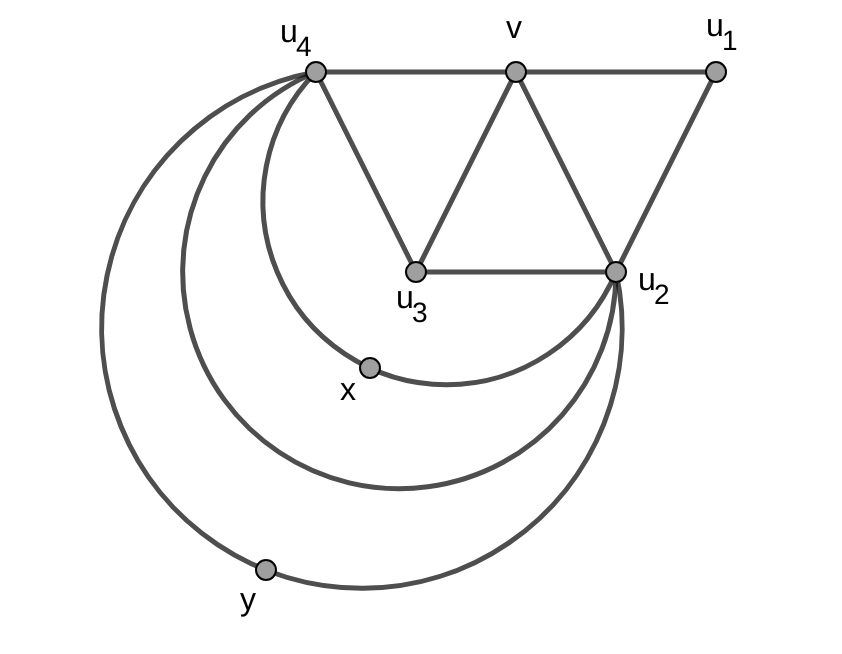
\includegraphics[width=70mm]{trans}
  \caption{Lemma \ref{l:trans}}
  \label{fig:trans}
\end{figure}

\begin{thm}
  $H$ is connected.
\end{thm}
\begin{proof}
  The proof goes as follows. First, we fix an $r$-rooted triangulation $t^*$. Then
  for every $t \in T$, we construct a path starting from $t$. Finally,
  we show that each of these paths ends in $t^*$.

  Define $t^*$ as follows. $v_1, v_2 \dots, v_r$ form the outer face of $t^*$.
  Connect $v_{r+1}$ to all the vertices of the outer face. For $i \ge r + 2$,
  put $v_i$ on the $v_{r-1}v_rv_{i-1}$ face and connect it with all of these three vertices.
  (See figure \ref{fig:root}.)

  \begin{figure}[ht]
    \centering
    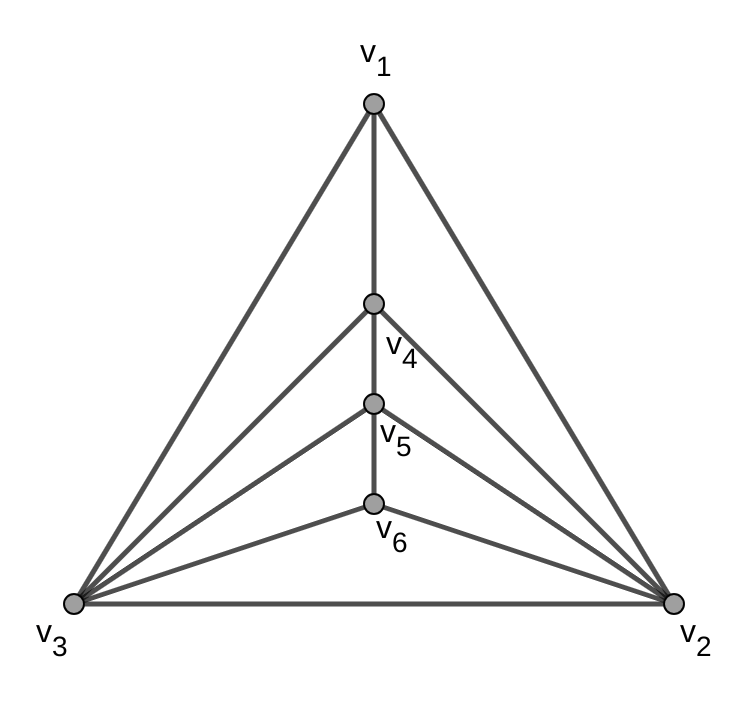
\includegraphics[width=70mm]{root}
    \caption{$t^*$ for $r=3$, $n = 6$}
    \label{fig:root}
  \end{figure}

  Let $t = (G, v_1, \dots v_r)$ be an $r$-rooted triangulation. We show now that
  Algorithm \ref{alg:path} stops in finitely many steps and constructs a path
  starting in $t$ and ending in $t^*$. Note, that when the algorithm flips an
  edge, then it is really transformable.
  \begin{algorithm}
    \caption{Construct path} \label{alg:path}
    \begin{algorithmic}
      \STATE let $p$ be an array of length $n$ /* $p[i]$ will be the $i^{th}$ vertex of the path.
      \STATE $p[0] := t$
      \WHILE{\TRUE}
        \STATE $j := j + 1$
        \STATE $i := 1$
        \WHILE{$deg(v_i) = 3$ and $i \le r - 2$}
          \STATE $i := i + 1$
        \ENDWHILE
        \IF{$i \le r - 2$}
          \STATE /* The outer face of $t$ differs from the outer face of $t^*$.
          \STATE let $v_{i - 1}, u_2, u_3, u_4$ be consecutive neighbors of $v_i$ in
          counterclockwise order
          \IF{$u_2u_4 \not\in E$}
            \STATE $p[j] := flip(t, v_iu_3)$
          \ELSE
            \STATE $p[j] := flip(t, u_2u_4)$
          \ENDIF
        \ELSE
          \STATE /* The outer face looks good, identify the possible $v_{r+1}$.
          \STATE let $w$ be the vertex connected to $v_1, \dots v_{r - 2}$.
          \STATE $a = v_1$
          \WHILE{$w$ has exactly one neighbor $b \neq a$ not on the outer face of  $t$}
            \STATE /* If $w$ was the possible $v_k$, then $b$ is the possible $v_{k + 1}$.
            \STATE $a = w$
            \STATE $w = b$
          \ENDWHILE
          \IF{$deg(w) = 3$}
            \STATE return $p$
          \ELSE
            \STATE let $v_r, u_2, u_3, u_4$ be consecutive neighbors of $w$ in
            counterclockwise order
            \IF{$u_2u_4 \not\in E$}
              \STATE $p[j] := flip(t, wu_3)$
            \ELSE
              \STATE $p[j] := flip(t, u_2u_4)$
            \ENDIF
          \ENDIF
        \ENDIF
        \STATE $t := p[j]$
      \ENDWHILE
    \end{algorithmic}
  \end{algorithm}

  We claim that after enough steps, $deg(v_1) = \dots = deg(v_{r - 2}) = 3$.
  Suppose that $deg(v_i) \neq 3$ for some $i \le r - 2$. Let $i$ be the smallest such index.
  Then the algorithm takes $v_{i - 1}, u_2, u_3, u_4$ such that they are consecutive neighbors of $v_i$
  in counterclockwise order. If $v_iu_3$ is transformable, then the degree of $v_i$
  decreases and for every $j < i, deg(v_j)$ does not change. Suppose that $v_iu_3$
  is not transformable. Then let $xu_2u_4$ and $yu_2u_4$ be the two faces bounding $u_2u_4$.
  Suppose $y = v_j$ for some $j < i$. From $deg(v_j) = 3$ it follows, that $u_4$ must be $v_{j - 1}$.
  On the other hand, by $3$-connectivity, if $u_4$ is an external vertex, then it
  is $v_{i + 1}$ and hence $i = r - 1$, which is a contradiction. So adding $xy$ to the graph
  does not change the degree of $v_j$ for any $j < i$. In the next step of the algorithm,
  $v_iu_3$ is transformable. So we showed, that after enough steps, $deg(v_i) = 3$ for every $i \le r - 2$.

  If $v_1, \dots v_{r - 2}$ are all degree $3$ vertices, then there exists a vertex $w$
  such that $w$ is connected to $v_1, \dots v_r$. If $w$ has
  more than one internal neighbor, than the algorithm chooses $v_r, u_2, u_3, u_4$ to
  be consecutive neighbors of $w$ in counterclockwise order. If $wu_3$ is transformable,
  then the algorithm deletes $wu_3$ from the graph and adds $u_2u_4$ to it. By executing this step,
  the degree of $w$ decreases, and for $j \le r - 2$, $deg(v_j)$ does not change.
  The other case is when $wu_3$ is not transformable. Let $x$ and $y$ be the
  vertices of the two faces bounded by $u_2u_4$, In this case the algorithm
  deletes $u_2u_4$ from the graph and adds $xy$ to the it. This does not change the
  degree of $v_j$ for $j \le r - 2$. In the next step of the algorithm $wu_3$ will be
  transformable. Thus, after some steps, $w$ will have only one internal neighbor $b$.
  It follows, that $bv_r$ and $bv_{r - 1}$ are edges. With the same process, we
  achieve that $b$ has at most $1$ internal neighbor apart from $v$. It is easy to see, that
  the changes does not affect vertices outside of $bv_rv_{r - 1}$. Thus, by iterating these
  steps we can achieve $t^*$.
\end{proof}

TODO: DFS,futasido


\addcontentsline{toc}{chapter}{Bibliography}
\begin{thebibliography}{9}

\bibitem{outerplanar}
Zoltán Lóránt Nagy
\textit{Coupon-coloring and total domination in Hamiltonian planar triangulations}
arXiv preprint arXiv:1708.01725

\bibitem{gh}
Wayne Goddard, Michael A. Henning
\textit{Thoroughly distributed colorings}
arXiv preprint arXiv:1609.09684

\bibitem{zelinka}
Bohdan Zelinka
\textit{Total domatic number and degree of vertices of a graph}.
Mathematica Slovaca, Vol. 39 (1989), No. 1, 7--11

\bibitem{np-complete}
Pinar Heggernes, Jan Arne Telle
\textit{Partitioning graphs into generalized dominating sets}
Nord. J. Comput. 5 (2), 128-142Nord. J. Comput. 5 (2), 128-142

\bibitem{regular}
H. Aram, S. M. Sheikholeslami, L. Volkmann
\textit{On the total domatic number of regular graphs}
Transactions on Combinatorics 1, 45-51

\bibitem{barnette}
David W. Barnette
\textit{Conjecture 5}
Recent progress in combinatorics (ed. W. T. Tutte), Academic Press, New York (1969) 343

\bibitem{spec_barnette}
Helmut Alt, Michael S. Payne, Jens M. Schmidt, David R. Wood
\textit{Thoughts on Barnette's conjecture}
arXiv preprint arXiv:1312.3783

\bibitem{ham1}
H. Whitney
\textit{A theorem on graphs}
Ann. Math. 32 (1931), 378-390

\bibitem{ham5}
Guido Helden
\textit{Hamiltonicity of maximal planar graphs and planar triangulations}
These de doctorat, RWTH Aachen University

\end{thebibliography}


\end{document}
